\section{HelloWorld for Java}

\subsection{Scope}

In this tutorial you will build your first very simple \eTrice{} model. The goal is to learn the work flow of 
\eTrice{} and to understand a few basic features of ROOM. You will perform the following steps:

\begin{enumerate}
\item create a new model from scratch
\item add a very simple state machine to an actor
\item generate the source code
\item run the model
\item open the message sequence chart
\end{enumerate}

Make sure that you have set up the workspace as described in \emph{Setting up the Workspace for Java}.

\subsection{Create a new model from scratch}

The easiest way to create a new \eTrice{} Project is to use the eclipse project wizard. From the eclipse file 
menu select \emph{File->New->Project} and create a new \emph{Empty eTrice Java Project} and name it \textbf{HelloWorld}.

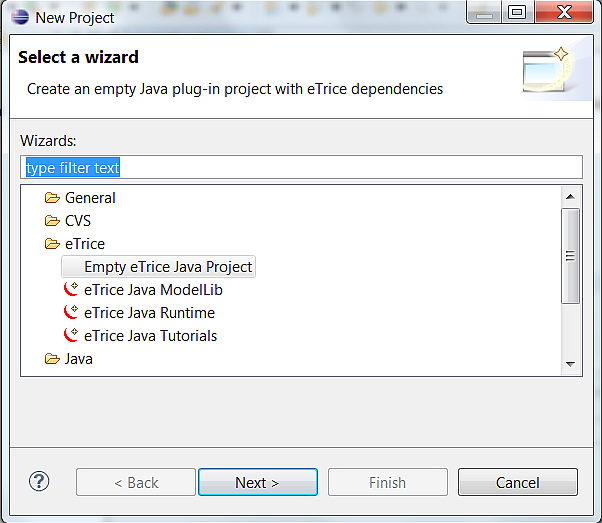
\includegraphics[width=0.8\textwidth]{images/015-HelloWorld10.png}

The wizard creates everything that is needed to create, build and run an \eTrice{} model. The resulting 
project should look like this:

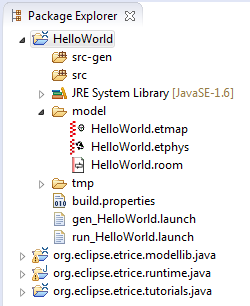
\includegraphics{images/015-HelloWorld11.png}

Within the model directory the model file \emph{HelloWorld.room} was created. Open the 
\emph{HelloWorld.room} file and delete the contents of the file. Open the content assist with Ctrl+Space 
and select \emph{RoomModel - model skeleton}.

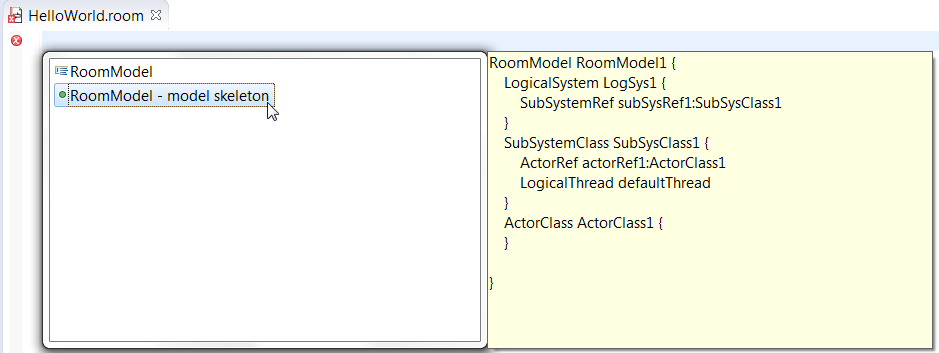
\includegraphics[width=0.6\textwidth]{images/015-HelloWorld12.png}

Edit the template variables by typing the new names and jumping with Tab from name to name.

The resulting model code should look like this:

\begin{lstlisting}[language=ROOM]
RoomModel HelloWorld_Model {

	LogicalSystem LogSys1 {
		SubSystemRef subSysRef1: SubSysClass1
	}

	SubSystemClass SubSysClass1 {
		ActorRef actorRef1: HelloWorldTop
		LogicalThread defaultThread
	}

	ActorClass HelloWorldTop { }

}
\end{lstlisting}

The physical model has already been created for us in file model/HelloWorld.etphys.
We can just leave it as it is.

\begin{lstlisting}[language=etPhys]
PhysicalModel PhysicalModel1 {

	PhysicalSystem PhysSys1 {
		NodeRef nodeRef1 : NodeClass1
	}

	NodeClass NodeClass1 {
		runtime = RuntimeClass1
		priomin = -10
		priomax = 10
		DefaultThread PhysicalThread1 {
			execmode = mixed
			interval = 100 ms
			prio = 0
			stacksize = 1024
			msgblocksize = 32
			msgpoolsize = 10
		}
	}

	RuntimeClass RuntimeClass1 {
		model = multiThreaded
	}
}
\end{lstlisting}

The physical model defines the setup of your nodes with their attributes like threads and mode of execution. In this case we define one node with one thread. 

Similar for the mapping model model/HelloWorld.etmap which is used to deploy the logical system onto the physical system.

\begin{lstlisting}[language=etMap]
MappingModel MappingModel1 {
	import HelloWorld_Model.* from "HelloWorldC.room"
	import PhysicalModel1.* from "HelloWorldC.etphys"
	Mapping LogSys1 -> PhysSys1 {
		SubSystemMapping subSysRef1 -> nodeRef1 {
			ThreadMapping defaultThread -> PhysicalThread1
		}
	}
}
\end{lstlisting}

The goal of \eTrice{} is to describe distributed systems on a logical level. In the current version not all 
elements will be used. But as prerequisite for further versions the following elements can be defined:
\begin{itemize}
\item the \textit{LogicalSystem} (currently optional)
\item at least one \textit{SubSystemClass} (mandatory)
\item at least one \textit{ActorClass} (mandatory)
\end{itemize}

The \textit{LogicalSystem} represents the complete distributed system and contains at least one 
\textit{SubSystemRef}. The \textit{SubSystemClass} represents an address space (e.g. a linux process or an image for a microcontroller) and contains at least one 
\textit{ActorRef}. The \textit{ActorClass} is the building block for building the hierachical structure of an application. 
A good point to start is to define a top level actor that can be used as structural root within the subsystem.

The outline view of the textual ROOM editor shows the main modeling elements in a navigation tree. You can jump to an element in the textual editor by double clicking the element in the outline view.

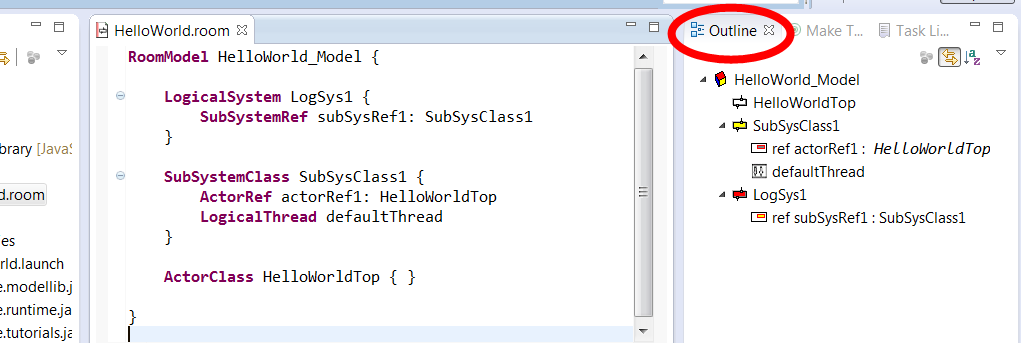
\includegraphics[width=0.8\textwidth]{images/015-HelloWorld02.png}
% !images/015-HelloWorld02.png!

\subsection{Create a state machine}

We will implement the Hello World code on the initial transition of the \textit{HelloWorldTop} actor. 
Therefore open the state machine editor by right clicking the \textit{HelloWorldTop} actor in the outline view and select \textit{Edit Behavior}.

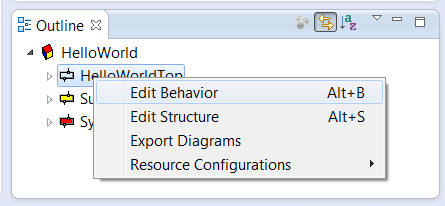
\includegraphics{images/015-HelloWorld03.png}
% !images/015-HelloWorld03.png!

The state machine editor will be opened. Drag and drop an \textit{Initial Point} from the tool box to the 
diagram into the top level state. Drag and drop a \textit{State} from the tool box to the diagram. Confirm the dialogue with \textit{ok}. Select the \textit{Transition} in the tool box and draw the transition from the \textit{Initial Point} to the State. Open the transition dialogue by double clicking the transition arrow and fill in the action code. Be aware of the different action code in Java and C.

\begin{figure}[ht]
\begin{minipage}[b]{0.45\linewidth}
	\begin{mdframed}
	\textbf{action code for Java}
	\begin{verbatim}
	System.out.println("Hello World !");
	\end{verbatim}
	\end{mdframed}
\end{minipage}
\hspace{0.5cm}
\begin{minipage}[b]{0.45\linewidth}
	\begin{mdframed}
	\textbf{action code for C}
	\begin{verbatim}
	printf("Hello World\n");
	\end{verbatim}
	\end{mdframed}
\end{minipage}
\end{figure}

 
The result should look like this:

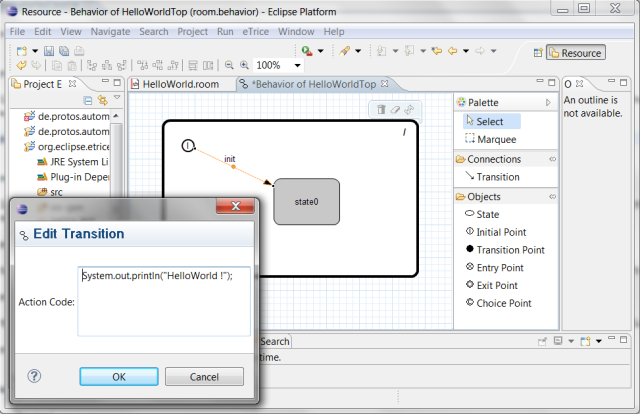
\includegraphics[width=0.8\textwidth]{images/015-HelloWorld04.png}
% !images/015-HelloWorld04.png!

Save the diagram and inspect the model (HelloWorld.room) file. Note that the textual representation was changed after saving 
the diagram.

\begin{figure}[ht]
\begin{minipage}[t]{0.50\linewidth}
\begin{mdframed}
	\textbf{room model for Java}
	\newline
\begin{lstlisting}[language=ROOM]
RoomModel HelloWorld_Model {
	LogicalSystem LogSys1 {
		SubSystemRef subSysRef1:SubSysClass1 
	}
	SubSystemClass SubSysClass1 {
		ActorRef actorRef1:HelloWorldTop 
		LogicalThread defaultThread
	}
	ActorClass HelloWorldTop {
		Structure { }
		Behavior {
			StateMachine {
				Transition init: initial -> state0 {
					action {
						"System.out.println(\"Hello World\");"
					}
				}
				State state0
			}
		}
	}
}
\end{lstlisting}
\end{mdframed}
\end{minipage}
\hspace{0.1cm}
\begin{minipage}[t]{0.50\linewidth}
\begin{mdframed}
	\textbf{room model for C}
	\newline
\begin{lstlisting}[language=ROOM]
RoomModel HelloWorld_Model {
	LogicalSystem LogSys1 {
		SubSystemRef subSysRef1: SubSysClass1
	}
	SubSystemClass SubSysClass1 {
		ActorRef actorRef1: HelloWorldTop
		LogicalThread defaultThread
	}
	ActorClass HelloWorldTop {
		Structure { }
		Behavior {
			StateMachine {
				Transition init: initial -> state0 {
					action {
						"printf(\"Hello World\\n\");"
					}
				}
				State state0
			}
		}
	}
}
\end{lstlisting}
\end{mdframed}
\end{minipage}
\end{figure}





\subsection{Build and run the model}

Now the model is finished and the source code can be generated. The project wizard has created a launch 
configuration that is responsible for generating the source code. In the project \textit{HelloWorld} right click \emph{gen\_HelloWorld.launch} and run it as \emph{gen\_HelloWorld}. 

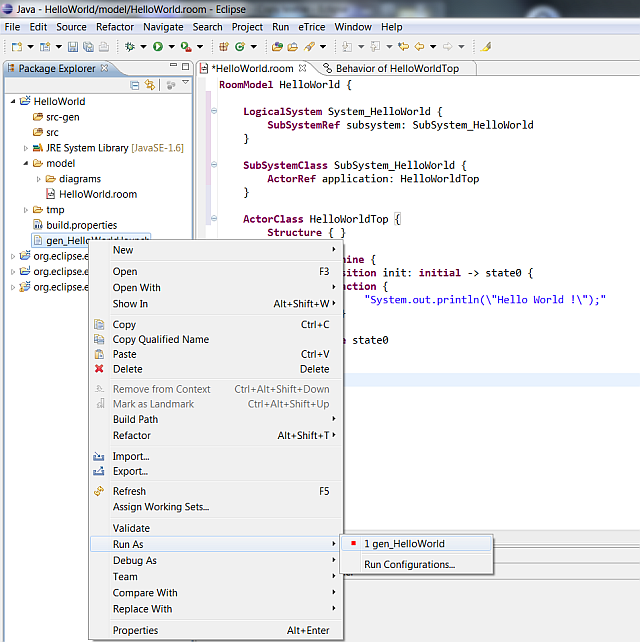
\includegraphics[width=0.8\textwidth]{images/015-HelloWorld06.png}

The source code for the model will be generated into the folder \emph{src-gen}. The main function will be contained in \emph{HelloWorld/Nod\_nodeRef1\_subSysRef1Runner.java}.
Select this file and run it as Java application or use the generated launch configuration \emph{run\_HelloWorld.launch}.

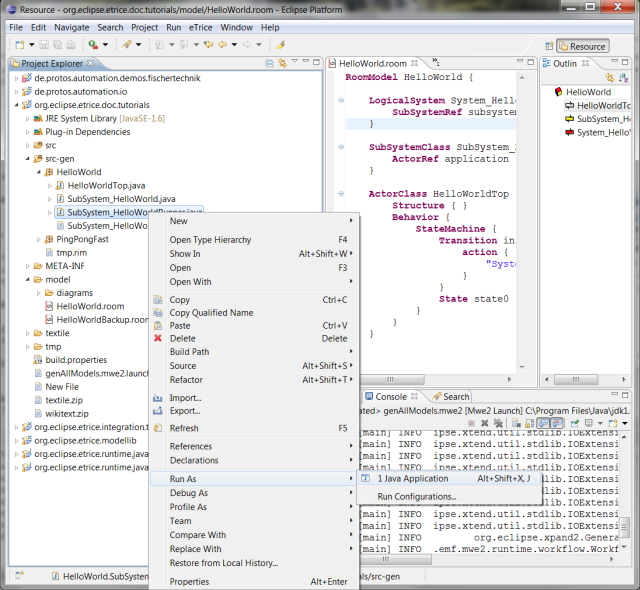
\includegraphics{images/015-HelloWorld07.png}


The Hello World application starts and the string \emph{"Hello World"} will be printed into the console window. To terminate the application the user must enter \emph{quit} in the console window.

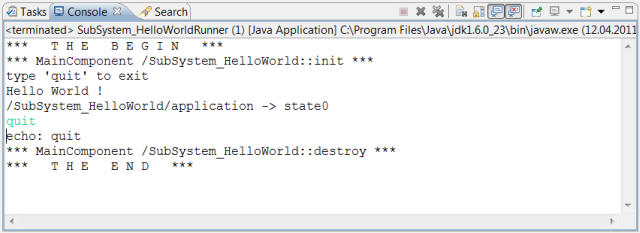
\includegraphics[width=0.6\textwidth]{images/015-HelloWorld08.png}

\subsection{Open the Message Sequence Chart}

For debugging and learning purposes, the application produced a Message Sequence Chart and wrote it to a file. Open the file \emph{subSysRef1\_Async.seq} or \emph{msc.seq} in the folder \emph{HelloWorld/tmp/log/} using the tool Trace2UML. Create the path if not already there.

Trace2UML is an open source MSC viewer and can be obtained here:
\begin{itemize}
\item \href{http://trace2uml.tigris.org/}{Trace2UML project home and download of windows version} 
\item \href{http://apt.astade.de/}{download of the Linux package of the Astade UML tool which contains Trace2UML}
\end{itemize}
After opening the file, you should see something like this:

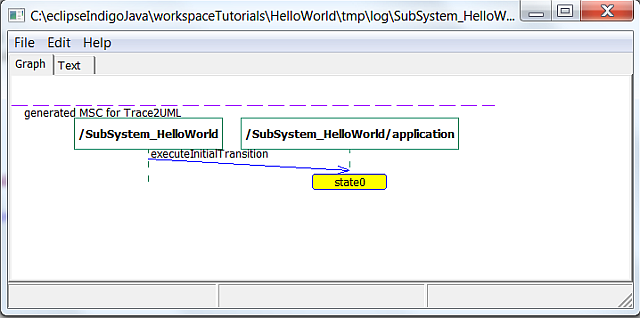
\includegraphics[width=0.6\textwidth]{images/015-HelloWorld09.png}
% !images/015-HelloWorld09.png!

The Actor with the instance path \emph{/LogSys1/subSysRef1/actorRef1} is in the state \emph{state0}. 
This is the simplest possible MSC. The MSCs for further tutorials will contain more information.


\subsection{Summary}

Now you have generated your first \eTrice{} model from scratch. You can switch between diagram editor and 
textual model representation (.room file) and you can see what will be generated during editing and saving the diagram files. 
You should take a look at the generated source files to understand how the state machine is generated and 
the life cycle of the application works. The next tutorials will deal with more complex hierarchies in structure and behavior.
